\begin{figure}[H]
\begin{center}
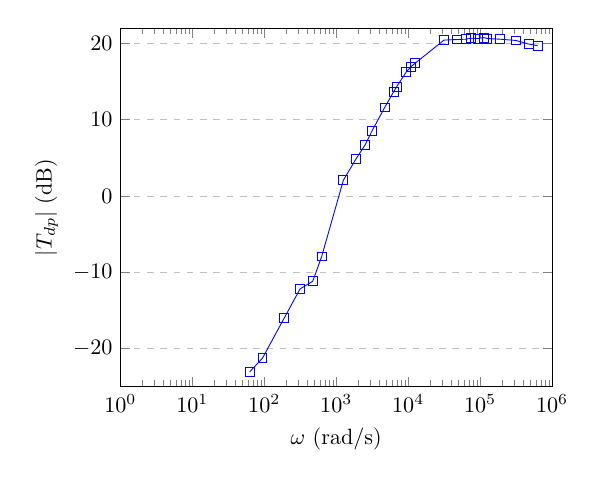
\begin{tikzpicture} [scale=0.8]
\begin{semilogxaxis}[
    title={},
    xlabel={$\omega$ (rad/s)},
    ylabel={$|T_{dp}|$ (dB)},
    xmin=1, xmax=1000000,
    ymin=-25, ymax=22,
    xtick={1,10,100,1000,10000,100000,1000000},
    ytick={-20,-10,0,10,20},
    legend pos=north west,
    ymajorgrids=true,
    grid style=dashed,
]
\addplot[
    color=blue,
    mark=square,
    ]
    coordinates {
    (62.83,-23.036)
    (94.25,-21.26)
    (188.5,-16.027)
    (314.16,-12.181)
    (471.24,-11.182)
    (628.32,-7.915)
    (1256.64,2.067)
    (1884.96,4.867)
    (2513.27,6.676)
    (3141.59,8.519)
    (4712.39,11.598)
    (6283.19,13.654)
    (6911.5,14.32)
    (9424.78,16.258)
    (10995.57,16.964)
    (12566.37,17.415)
    (31415.93,20.428)
    (47123.89,20.506)
    (62831.85,20.547)
    (75398.22,20.678)
    (94247.78,20.634)
    (113097.34,20.759)
    (125663.71,20.634)
    (188495.56,20.547)
    (314159.27,20.382)
    (471238.9,19.914)
    (628318.53,19.697)
    };
\end{semilogxaxis}
\end{tikzpicture}
\hspace{1cm}
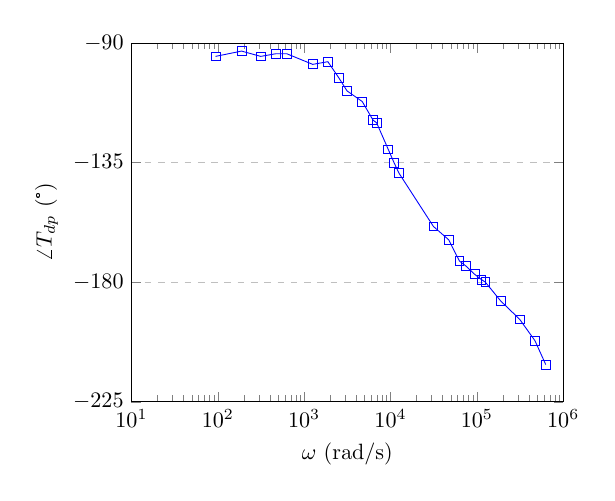
\begin{tikzpicture} [scale=0.8]
\begin{semilogxaxis}[
    title={},
    xlabel={$\omega$ (rad/s)},
    ylabel={$\angle T_{dp}$ (°)},
    xmin=10, xmax=1000000,
    ymin=-225, ymax=-90,
    xtick={10,100,1000,10000,100000,1000000},
    ytick={-225, -180, -135, -90},
    legend pos=north west,
    ymajorgrids=true,
    grid style=dashed,
]
\addplot[
    color=blue,
    mark=square,
    ]
    coordinates {
    (94.25,-95)
    (188.5,-93)
    (314.16,-95)
    (471.24,-94)
    (628.32,-94)
    (1256.64,-98)
    (1884.96,-97)
    (2513.27,-103)
    (3141.59,-108)
    (4712.39,-112)
    (6283.19,-119)
    (6911.5,-120)
    (9424.78,-130)
    (10995.57,-135)
    (12566.37,-139)
    (31415.93,-159)
    (47123.89,-164)
    (62831.85,-172)
    (75398.22,-174)
    (94247.78,-177)
    (113097.34,-179)
    (125663.71,-180)
    (188495.56,-187)
    (314159.27,-194)
    (471238.9,-202)
    (628318.53,-211)
    };
\end{semilogxaxis}
\end{tikzpicture}
\end{center}
\caption{Curvas de bode com os resultados práticos da função de transferência do derivador.}
\label{graph:2} 
\end{figure}